% Figures 1-6 (from scripts/make_paper_figures.py). Floats; LaTeX places them near Section 5.

\begin{figure}[tbp]
  \centering
  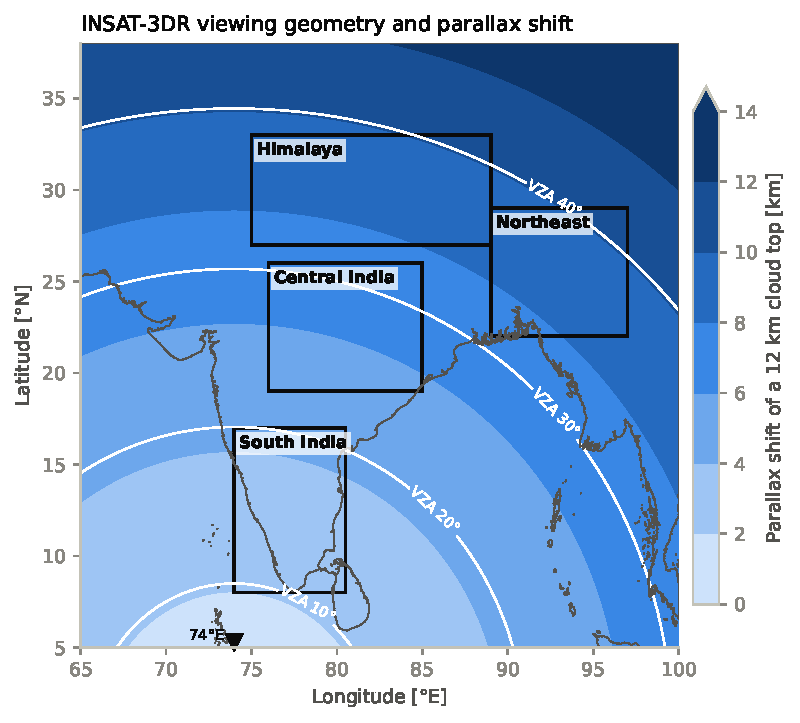
\includegraphics[width=0.8\textwidth]{figures/fig1_geometry.pdf}
  \caption{INSAT-3DR viewing geometry over South Asia. Colours: parallax shift of a 12\,km cloud top, $h\tan(\mathrm{VZA})$; white lines: viewing zenith angle. Boxes: the four validation regions. The sub-satellite point is at 74\,\textdegree E.}
  \label{fig:1}
\end{figure}

\begin{figure}[tbp]
  \centering
  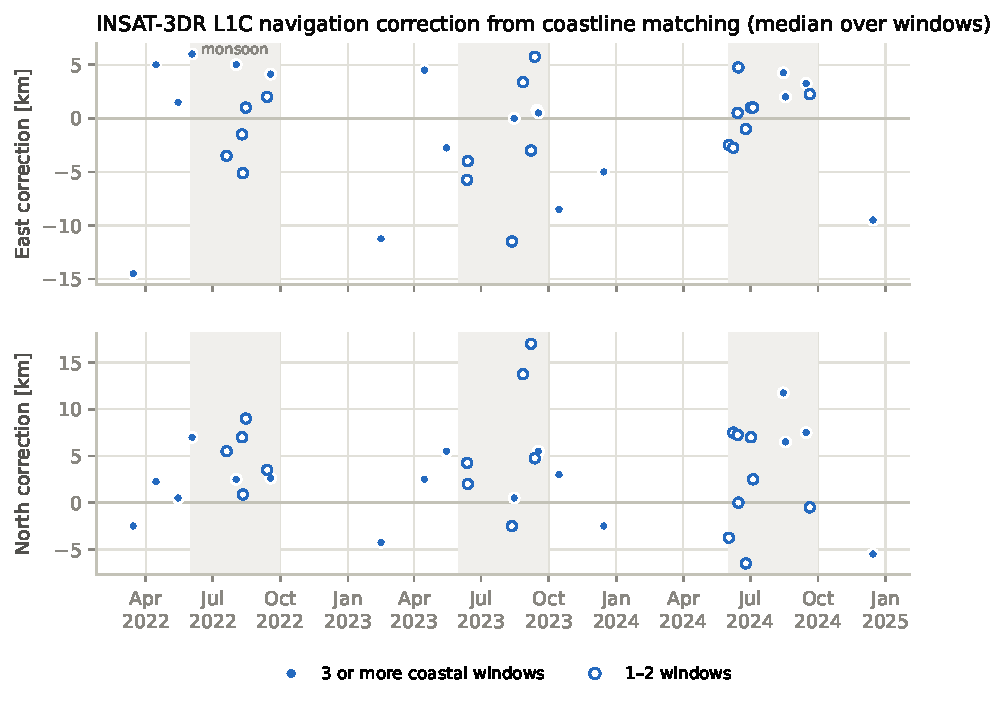
\includegraphics[width=\textwidth]{figures/fig2_navigation.pdf}
  \caption{INSAT-3DR L1C navigation correction from coastline matching, March 2022 to December 2024 (median over the accepted coastal windows of each date). Filled points: three or more windows; open points: one or two. Shading: June--September. Positive values mean INSAT positions must move east or north.}
  \label{fig:2}
\end{figure}

\begin{figure}[tbp]
  \centering
  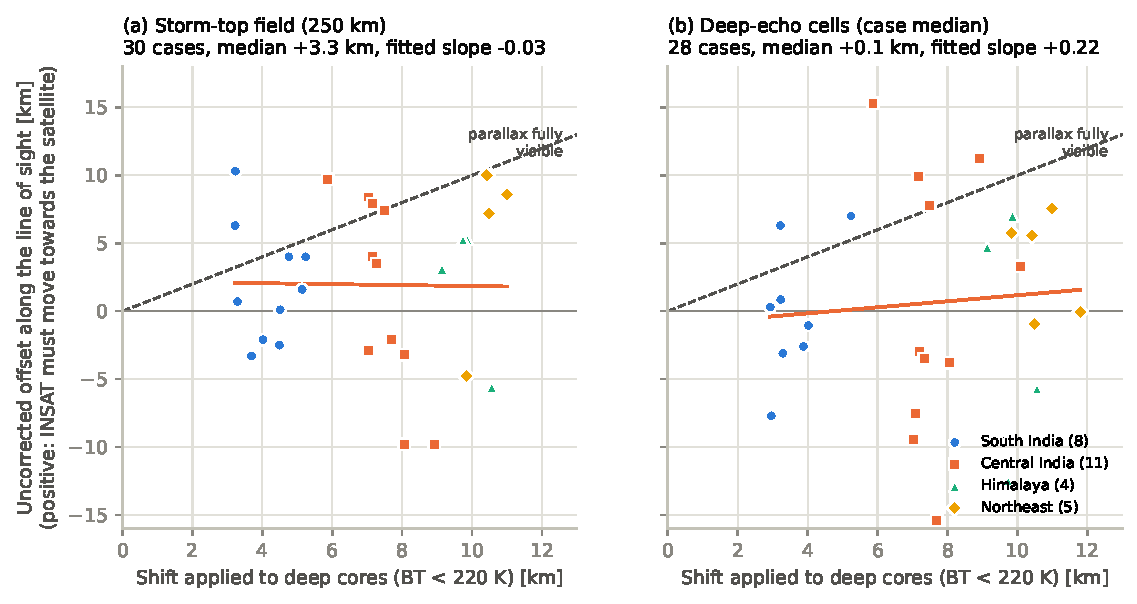
\includegraphics[width=0.9\textwidth]{figures/fig3_cases.pdf}
  \caption{Line-of-sight offset between INSAT and GPM (storm-top field, 250\,km window) for each case before (open) and after (filled) parallax correction, ordered by viewing zenith angle (in brackets). Positive: INSAT must move towards the satellite to match GPM.}
  \label{fig:3}
\end{figure}

\begin{figure}[tbp]
  \centering
  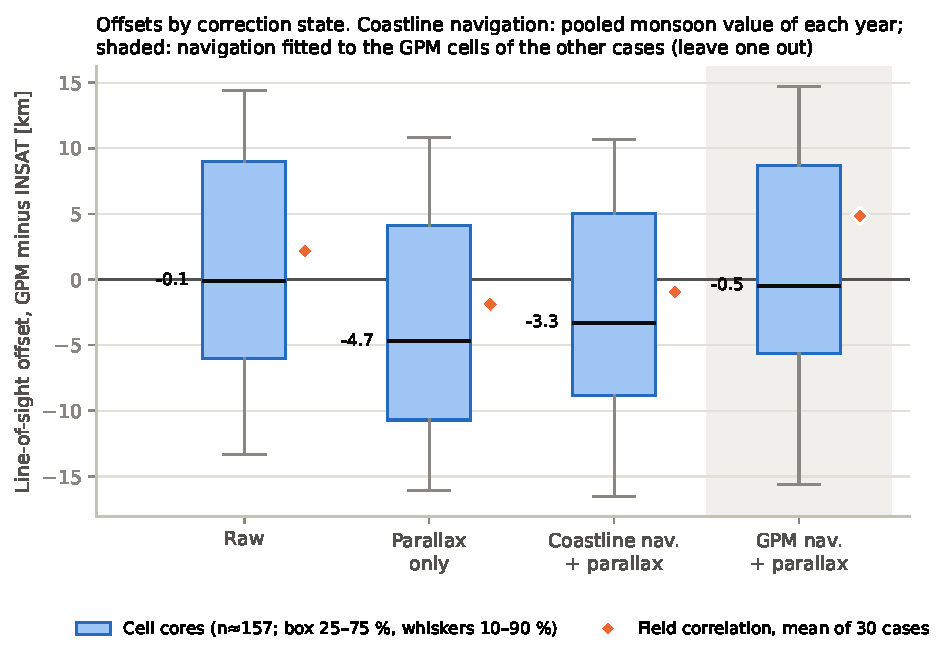
\includegraphics[width=\textwidth]{figures/fig4_states.pdf}
  \caption{Line-of-sight offsets in each correction state. Boxes: cell-by-cell offsets between GPM deep-echo cells and INSAT cold cores (box 25--75\,\%, whiskers 10--90\,\%; median labelled). Diamonds: mean field-correlation offset over 12 cases. Navigation: near-storm monsoon correction ($-0.5$\,km E, $+2.5$\,km N); shaded: all-India monsoon median ($+1.8$\,km E, $+4.8$\,km N) as a sensitivity test.}
  \label{fig:4}
\end{figure}

\begin{figure}[tbp]
  \centering
  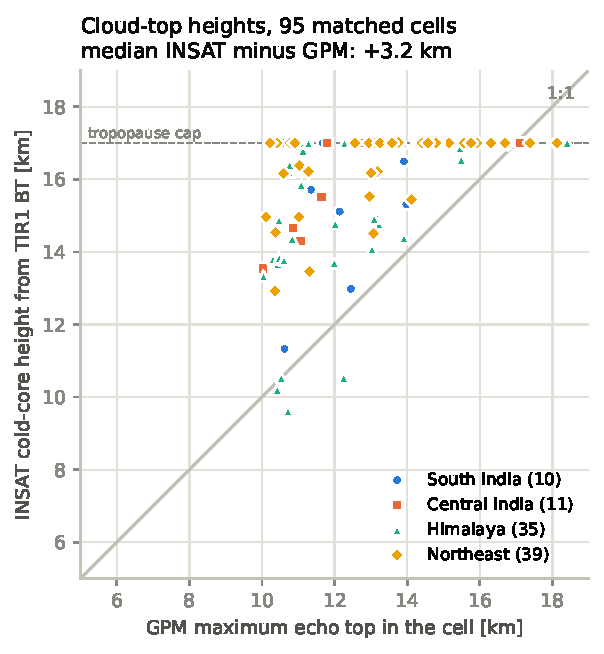
\includegraphics[width=0.6\textwidth]{figures/fig5_heights.pdf}
  \caption{Cloud-top height of the INSAT cold core (from TIR1 brightness temperature, AFGL tropical profile) against the GPM maximum echo top in the same cell, for 95 matched cells. Dashed line: the tropopause cap of the profile.}
  \label{fig:5}
\end{figure}

\begin{figure}[tbp]
  \centering
  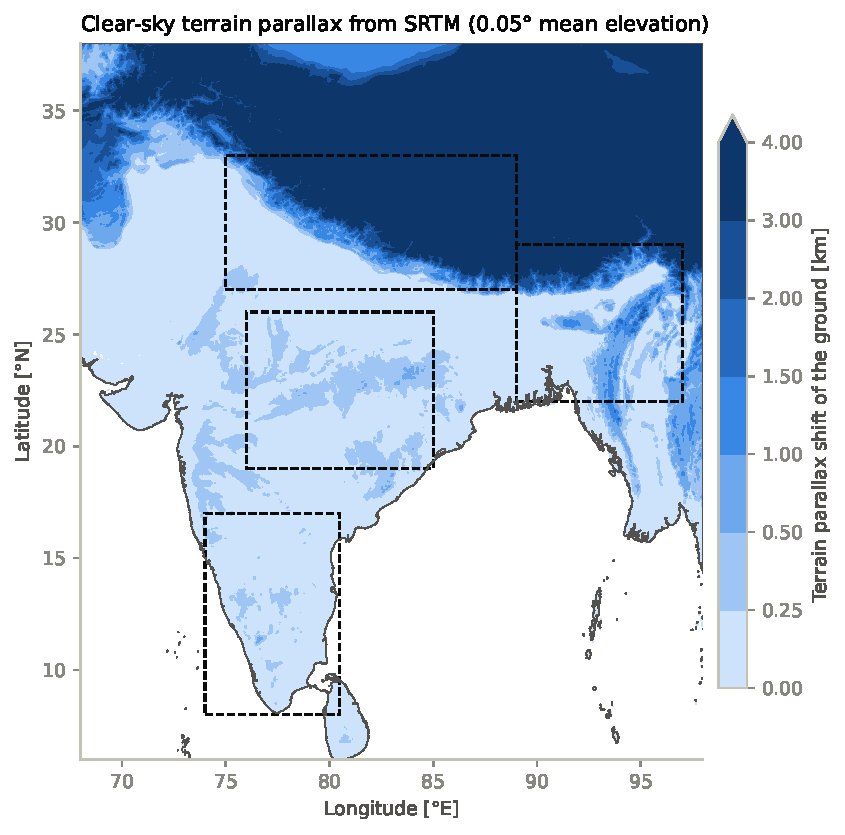
\includegraphics[width=0.8\textwidth]{figures/fig6_terrain.pdf}
  \caption{Clear-sky terrain parallax: displacement of the ground in ellipsoid-navigated INSAT-3DR imagery, from SRTM elevation averaged to 0.05\,\textdegree. Dashed boxes: validation regions.}
  \label{fig:6}
\end{figure}
